% ----------------------------------------------------------------------------------------
%	PACKAGES AND THEMES
% ----------------------------------------------------------------------------------------
\documentclass[aspectratio=169,xcolor=dvipsnames, t]{beamer}
\usepackage{fontspec} % Allows using custom font. MUST be before loading the theme!
\usetheme{SimplePlusAIC}
\usepackage{ulem} 
\usepackage{hhline}
\usepackage{hyperref}
\usepackage{graphicx} % Allows including images
\usepackage{booktabs} % Allows the use of \toprule, \midrule and  \bottomrule in tables
\usepackage{svg} %allows using svg figures
\usepackage{tikz}
\usepackage{makecell}
\usepackage{amsmath} % For \textsubscript command
\usepackage[spanish]{babel}
\usepackage[backend=biber, style=apa]{biblatex}
\addbibresource{test.bib}
\usepackage{wrapfig}
% ADD YOUR PACKAGES BELOW
\usetikzlibrary{calc,patterns.meta}
\usepackage{totcount}
\regtotcounter{section}
\usepackage{forest}
\usepackage{colortbl}
\usepackage{color,soul}
\usepackage{xcolor}
\usepackage{nameref}

\synctex=1
% Redefinition of the \section command so that each one is labeled \label{sec:n} where n is its index 
\let\oldsection\section
\renewcommand{\section}[2][\relax]{%
  \ifx#1\relax
    \oldsection{#2}%
  \else
    \oldsection[#1]{#2}%
  \fi%
  \label{sec:\thesection}%
}

% Definition of custom colors based on the initial figure of the bar by the OP
\definecolor{myblue}{HTML}{57AED1}
\definecolor{mygreen}{HTML}{8BC53F}
\definecolor{mygray}{HTML}{DDDDDD}
\definecolor{BlueIuss}{HTML}{033354}
\definecolor{LightBlueIuss}{HTML}{1b4a74}

% Definition of custom tikz styles in order to ease readability
\tikzset{
  % Bar style (Argument : color)
  sectionbar/.style={
    % Filling with one color as a preaction, in order to avoid reset by the pattern color
    preaction={fill=#1!70},
    % Application of the line pattern on to of the fill
    pattern={Lines[angle=45,distance={6pt},line width=3pt]},pattern color=#1
  },
  % Node style (Arguments : color, section number)
  sectionnode/.style 2 args={
    fill=#1,
    draw=white,
    thick,
    circle,
    text=white,
    radius=10pt,
    % Display of the section name below the cicle
    label={[text=#1, text width=2cm, align=center]below:\nameref{sec:#2}},
  }
}


% Actual definition of the colorbar based on Gonzalo Medina's initial proposal
\makeatletter
\def\pbar@progressbar{} % the progress bar
\newcount\pbar@tmpcnta% auxiliary counter
\newcount\pbar@tmpcntb% auxiliary counter
\newdimen\pbar@pbht %progressbar height
\newdimen\pbar@pbwd %progressbar width
\newdimen\pbar@tmpdim % auxiliary dimension
\pbar@pbwd=\linewidth
\pbar@pbht=4pt

% The progress bar
\def\pbar@progressbar{%
  \pbar@tmpcnta=\value{section} % tmpcnta stores the section number
  \pbar@tmpcntb=\totvalue{section} % tmbcountb sotres the total amount of sections
  \advance\pbar@tmpcntb by 1 % tmbcountb is advanced by 1 in order to have the last bar segment after the last node

  \begin{tikzpicture}[very thin]
    % Clipping scope to avoid tests for the bar dimensions
    \begin{scope}
      % Clipping path
      \path[rounded corners=2pt,clip] (0pt,{-\pbar@pbht/2}) rectangle (\pbar@pbwd,{\pbar@pbht/2});
      % Gray bar (from 0 to last section)
      \path[sectionbar=mygray] (0pt,{-\pbar@pbht/2}) rectangle (\linewidth,{\pbar@pbht/2});
      % Blue bar (from 0 to the current section)
      \path[sectionbar=BlueIuss] (0pt,{-\pbar@pbht/2}) rectangle ({(\pbar@tmpcnta-0.5)*\linewidth/\pbar@tmpcntb},{\pbar@pbht/2});
      % Green bar (from current to next section)
      \path[sectionbar=LightBlueIuss] ({(\pbar@tmpcnta-0.5)*\linewidth/\pbar@tmpcntb},{-\pbar@pbht/2}) rectangle ({(\pbar@tmpcnta+0.5)*\linewidth/\pbar@tmpcntb},{\pbar@pbht/2});
    \end{scope}
    % Drawing of the nodes on top of the bars, based on the number of the current section
    \foreach \secnumber in {1,...,\totvalue{section}}{
      % Number is lower, section is past, blue color
      \ifnum\secnumber<\pbar@tmpcnta
        \node[sectionnode={BlueIuss}{\secnumber}] at ({(\secnumber-0.5)*\linewidth/\pbar@tmpcntb},0) {\strut\secnumber};
      \fi
      % Number is equal, section is current, green color
      \ifnum\secnumber=\pbar@tmpcnta
        \node[sectionnode={LightBlueIuss}{\secnumber}] at ({(\secnumber-0.5)*\linewidth/\pbar@tmpcntb},0) {\strut\secnumber};
      \fi
      % Number is larger, to be done section, gray color
      \ifnum\secnumber>\pbar@tmpcnta
        \node[sectionnode={mygray}{\secnumber}] at ({(\secnumber-0.5)*\linewidth/\pbar@tmpcntb},0) {\strut\secnumber};
      \fi
    }
  \end{tikzpicture}%
}

\addtobeamertemplate{headline}{}
{%
  \begin{beamercolorbox}[wd=\paperwidth,ht=12.2ex,center,dp=1ex]{white}%
    \pbar@progressbar%
  \end{beamercolorbox}%
}
\makeatother

% ----------------------------------------------------------------------------------------
%	TITLE PAGE CONFIGURATION
% ----------------------------------------------------------------------------------------

\title[short title]{Point Visibility} % The short title appears at the bottom of every slide, the full title is only on the title page
% \subtitle{Subtitle}


\author{Arturo González Peñaloza\\ Dulce Julieta Mora Hernández}
\institute[Short title]{
  Universidad Nacional Autónoma de México
}
% Your institution as it will appear on the bottom of every slide, maybe shorthand to save space

\date{\today} % Date, can be changed to a custom date

% ----------------------------------------------------------------------------------------
%	PRESENTATION SLIDES
% ----------------------------------------------------------------------------------------

\begin{document}
\maketitlepage
% \section{Overview}
\begin{frame}[t]
  % Throughout your presentation, if you choose to use \section{} and \subsection{} commands, these will automatically be printed on this slide as an overview of your presentation
  \tableofcontents
\end{frame}

% -----------------------------------------------

% Section divider frame
\makesection{Introducción}
% \subsection{Entendiendo el problema}
\subsection{Definiciones Fundamentales}
\subsection{Algoritmo para cierre convexo en O(n)}

% ------------------------------------------------

\begin{frame}{Polígono de visibilidad}
  El \textit{polígono de visibilidad} $V(q)$ de un punto $q$ en un polígono simple $P$ es el conjunto de todos los puntos de $P$ que son visibles desde $q$.
  \begin{center}
    \begin{equation*}
      V(q) = \{ p \in P \text{ } | \text{ } q \text{ sees } p \}
    \end{equation*}
  \end{center}
\end{frame}

% ------------------------------------------------
% Tres columnas
\begin{frame}
  \begin{columns}[t]
    % Primera columna
    \begin{column}{0.33\textwidth}
      \begin{figure}
        \centering
        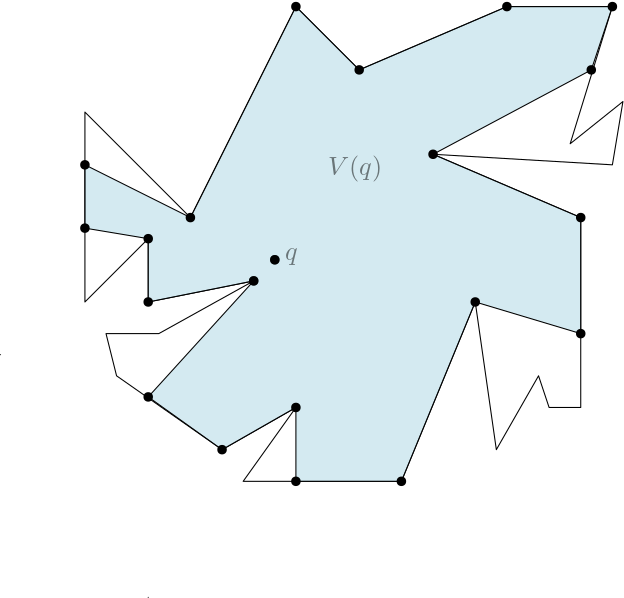
\includegraphics[width=0.9\textwidth]{imagenes/Case2.1a.png}
        \caption{Polígono simple}
      \end{figure}
    \end{column}

    % Segunda columna
    \begin{column}{0.33\textwidth}
      \begin{figure}
        \centering
        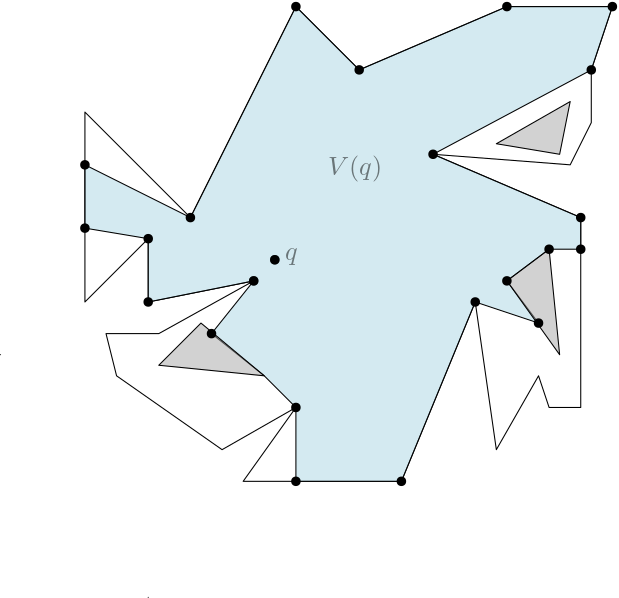
\includegraphics[width=0.9\textwidth]{imagenes/Case2.1b.png}
        \caption{Polígono con hoyos}
      \end{figure}
    \end{column}

    % Tercera columna
    \begin{column}{0.33\textwidth}
      \begin{figure}
        \hspace*{-1.5cm}
        \centering
        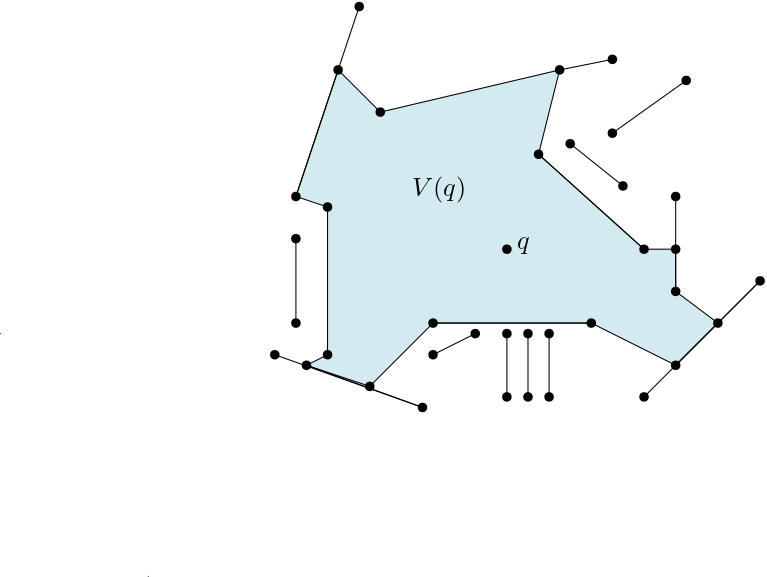
\includegraphics[width=1.15\textwidth]{imagenes/Caso2.1c.png}
        \caption{Conjunto de lineas}
      \end{figure}
    \end{column}
  \end{columns}
\end{frame}

% ------------------------------------------------
\begin{frame}{Arista construida}
  Sea $ab$ una arista en el perímetro de $V(q)$ de manera que
  \begin{columns}
    \begin{column}{0.45\textwidth}
      \begin{itemize}
      \item Ningún punto de $ab$, excepto $a$ y $b$, pertenecen al perímetro de $P$
      \item $q$, $a$ y $b$ son colineales
      \item $a$ o $b$ es un vértice de $P$\\
      \end{itemize}
      \vspace{0.5cm}
      \begin{center}
        La arista $ab$ se llama \textit{arista construida} de $V(q)$
      \end{center}
    \end{column}
    \begin{column}{0.45\textwidth}  %%<--- here
      \vspace{-1cm}
      % $uw$ es una arista de construcción
      \begin{wrapfigure}{l}{0.65\textwidth}
        \centering
        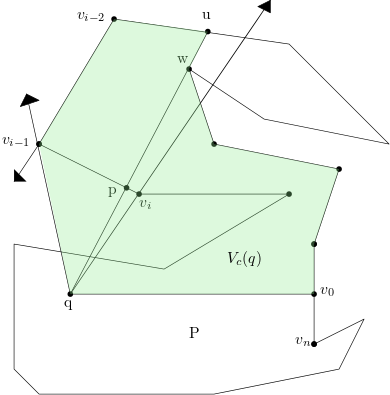
\includegraphics[width=0.65\textwidth]{imagenes/Caso2.7a.png}
        % \caption{}
      \end{wrapfigure}
    \end{column}
  \end{columns}
\end{frame}

% ------------------------------------------------

\begin{frame}[c]{Revoluciones}
  Para un polígono simple $P$ y un punto $z \in P$, el \textit{número de revoluciones} de $P$ con respecto a $z$ es el número de revoluciones que el perímetro de $P$ hace alrededor de $z$.\\
  \vspace{0.5cm}
  Si el número de revoluciones de $P$ respecto a $z$ es uno, $P$ es llamado \textit{non-winding polygon}.
\end{frame}

% ------------------------------------------------
% Double columns
\begin{frame}{}
  \begin{columns}
    \begin{column}{0.45\textwidth}
      El número de revoluciones de $P$ respecto a $q$ es dos
      \begin{wrapfigure}{c}{1.2\textwidth}
        \centering
        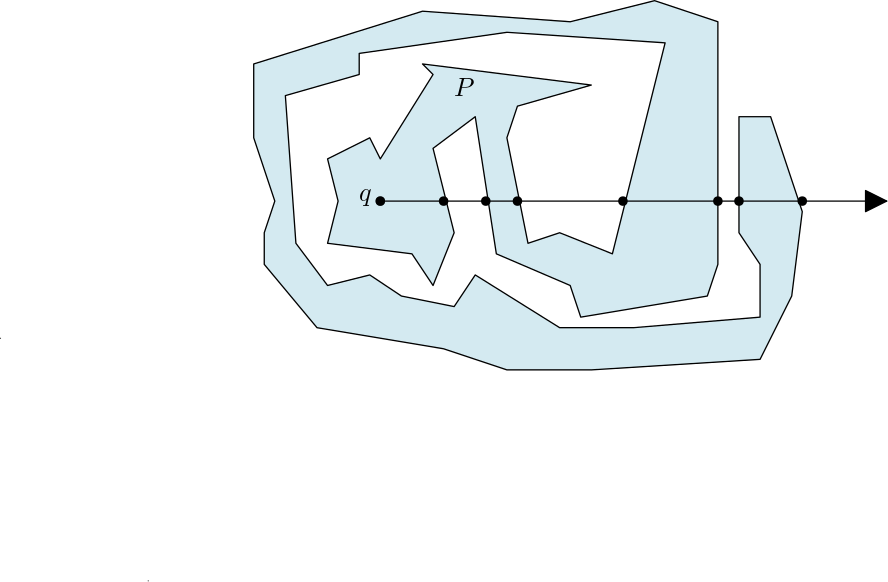
\includegraphics[width=1.2\textwidth]{imagenes/Case2.2a.png}
        % \caption{}
      \end{wrapfigure}
    \end{column}
    \begin{column}{0.45\textwidth}  %%<--- here
      El número de revoluciones de $P$ respecto a $q$ es una
      \begin{wrapfigure}{c}{1.2\textwidth}
        \centering
        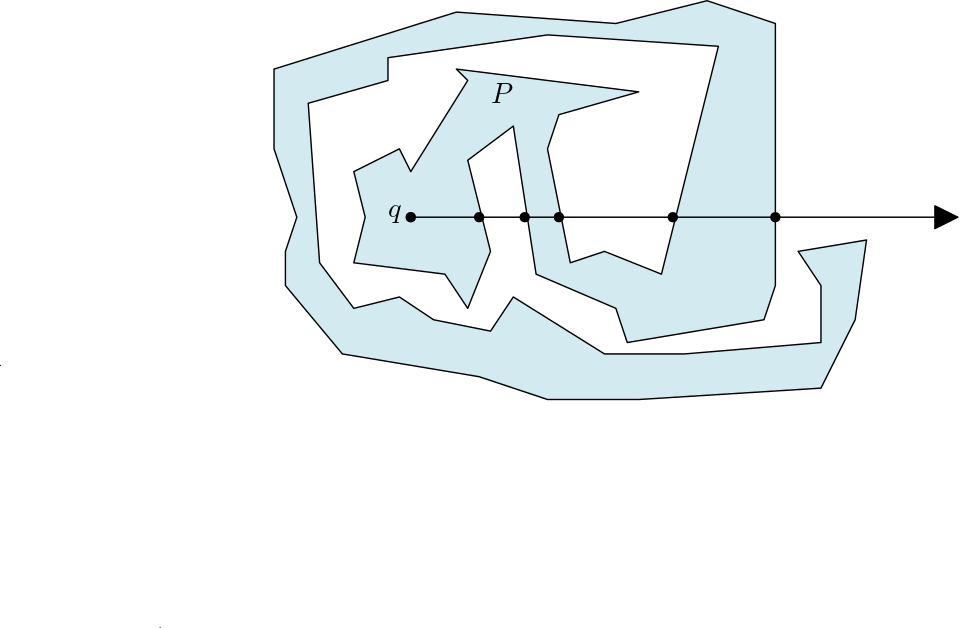
\includegraphics[width=1.2\textwidth]{imagenes/Caso2.2b.png}
        % \caption{}
      \end{wrapfigure}
    \end{column}
  \end{columns}
\end{frame}

% ------------------------------------------------
\subsection{Cierre Convexo en O(n)}
\begin{frame}{Algoritmo para calcular CH en O(n)}
  \begin{center}
    \begin{enumerate}
      \footnotesize
    \item t $\leftarrow$ -1; b $\leftarrow$ 0;\\
      $v_{1}$ $\leftarrow$ input; $v_{2}$ $\leftarrow$ input; $v_{3}$ $\leftarrow$ input;\\
      if ($v_{1}, v_{2}, v_{3}$) $>$ 0\\
      \hspace*{0.5cm} then begin push $v_{1}$; push $v_{2}$ ; end \\
      \hspace*{0.5cm} else begin push $v_{2}$; push $v_{1}$ ; end \\
      push $v_{3}$ ; insert $v_{3}$; 
    \item $v$ $\leftarrow$ input;\\
      until ($v$, $d_{b}$, $d_{b+1}$) < 0 or ($d_{t-1}, d_{t}, v) < 0$ \\
      \hspace*{0.5cm} do $v$ $\leftarrow$ input end;  
    \item until $(d_{t-1}, d_{t}, v) > 0$ do pop $d_{t}$ end;\\
      push $v$;
    \item until $(v, d_{b}, d_{b+1}) > 0$ do remove $d_{b}$ end;\\ 
      insert $v$; \\
      goto 2\\
    \end{enumerate}
  \end{center}
\end{frame}
\begin{frame}{Algoritmo de Melkman}
  Los polígonos simples simplifican el proceso de calcular su cierre convexo. El algoritmo de Melkman es una herramienta que aprovecha esta propiedad.
\end{frame}
\begin{frame}{Algoritmo de Melkman}
  \begin{enumerate}
  \item $D\gets (p_{2},p_{1},p_{1}) // $Se agregan a una deque dos puntos consecutivos del polígono.
  \item Para $i\gets 3$ a $n$ hacer:
    \begin{enumerate}
    \item Si $p_{i}$ está fuera del ángulo $v_{t-1}v_tv_{b+1}$, entonces
      \begin{enumerate}
      \item Mientras $p_{i}$ esté a la izquierda de $\overrightarrow{v_{b}v_{b+1}}$, entonces se saca desde abajo de $D$.
      \item Mientras $p_{i}$ esté a la derecha de $\overrightarrow{v_{t}v_{t-1}}$, entonces se saca desde arriba de $D$.
      \end{enumerate}
    \item Se agrega al inicio y al final de $D$ a $p_{i}$.
    \end{enumerate}
  \end{enumerate}
  \begin{block}{Observación}
    \small
    Si tomamos los primeros tres vértices de la deque (leidos de izquierda a derecha), obtenemos una vuelta a la derecha. Si tomamos los últimos tres vértices de la deque (leidos de derecha a izquierda), obtenemos una vuelta a la izquierda.
  \end{block}
\end{frame}
\begin{frame}{Ejemplo}
  \begin{figure}
    \centering
    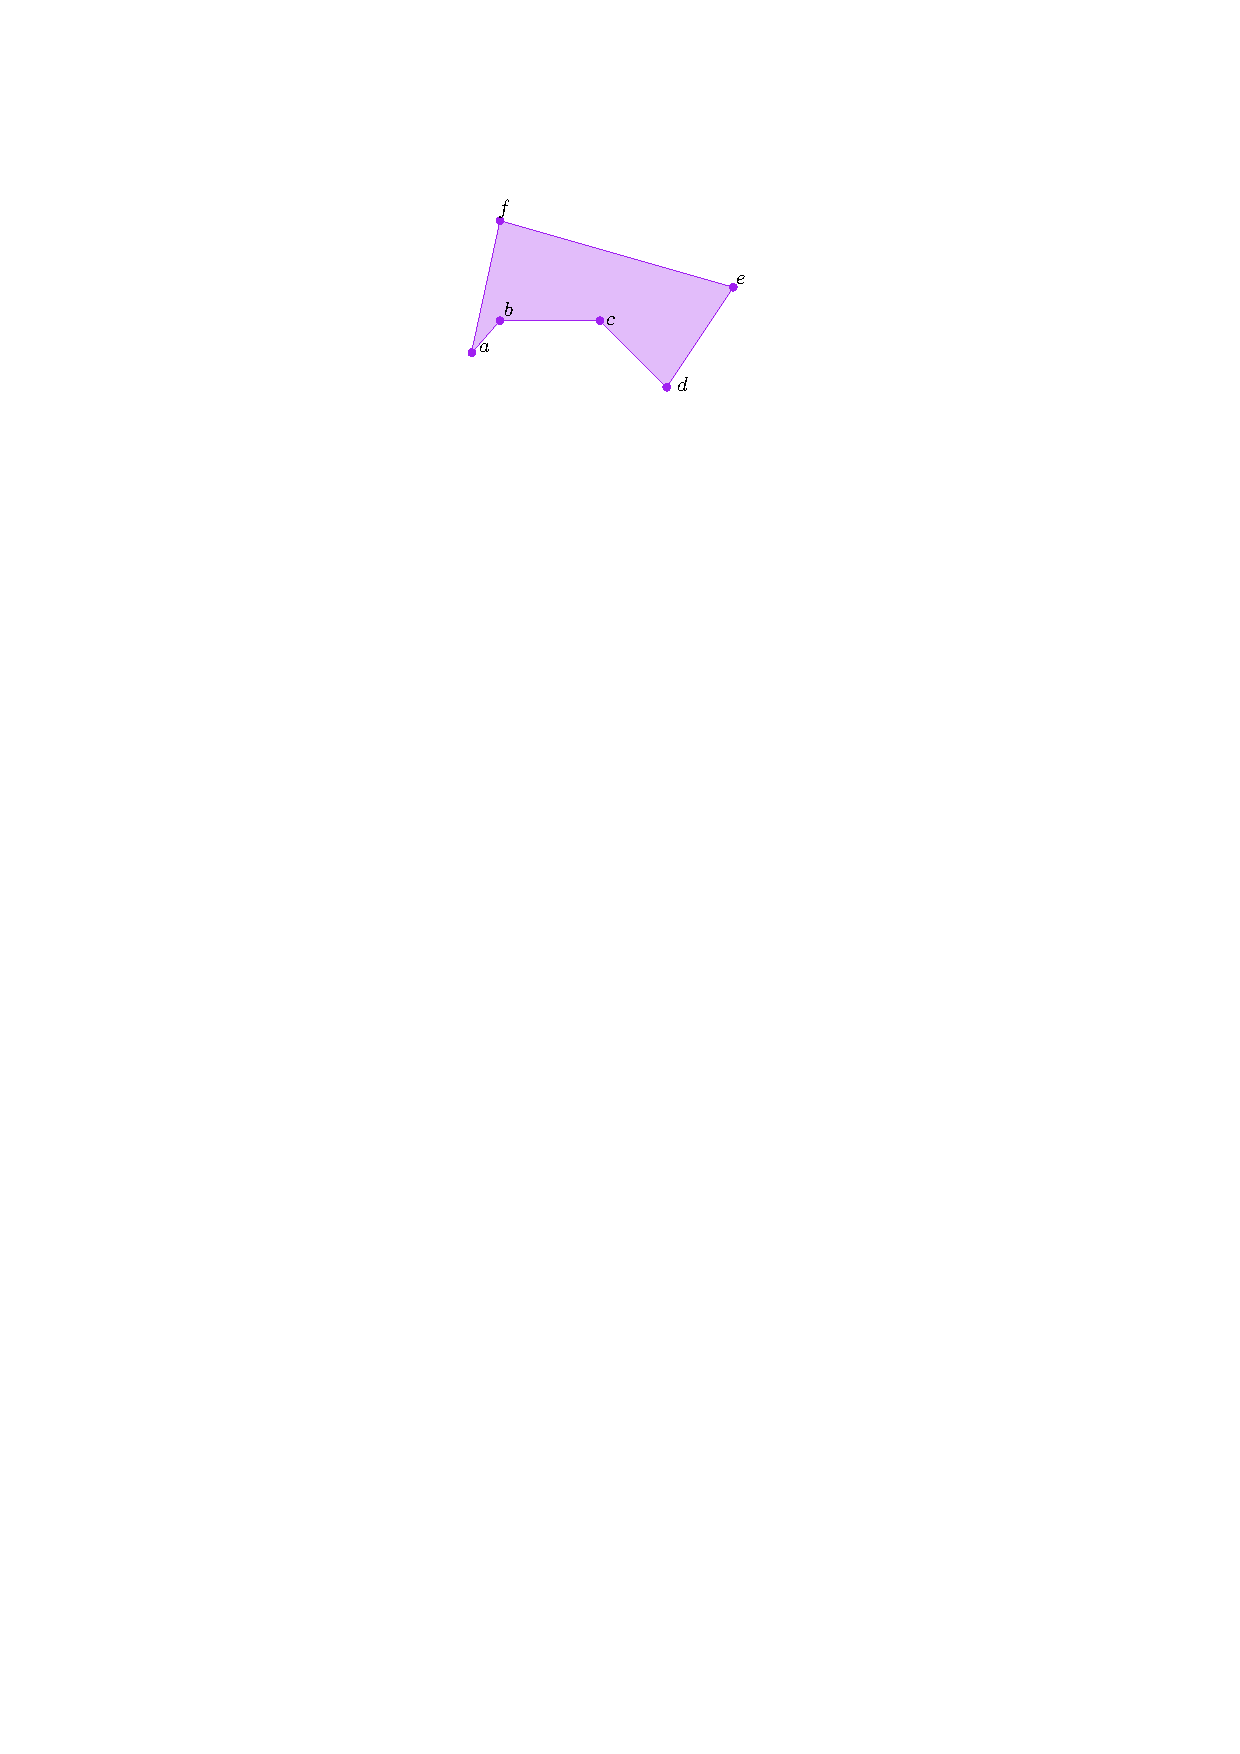
\includegraphics[width=\linewidth, height=0.5\textheight, page=1, keepaspectratio]{IPE/Melkman.pdf}
    \caption{Polígono simple}
  \end{figure}
\end{frame}
\begin{frame}{Ejemplo}
  \begin{figure}
    \centering
    \includegraphics[width=\linewidth, height=0.5\textheight, page=2, keepaspectratio]{IPE/Melkman.pdf}
    \caption{Polígono simple con su cierre convexo}
  \end{figure}
\end{frame}
\begin{frame}{Ejemplo}
  \begin{columns}
    \begin{column}{0.5\textwidth}
      Se agrega a la deque dos puntos consecutivos del polígono.
    \end{column}
    \begin{column}{0.5\textwidth}
      \begin{figure}
        \centering
        \includegraphics[width=\linewidth, height=0.5\textheight, page=3, keepaspectratio]{IPE/Melkman.pdf}
      \end{figure}
    \end{column}
  \end{columns}
  
\end{frame}
\begin{frame}{Ejemplo}
  \begin{columns}
    \begin{column}{0.5\textwidth}
      $c$ está a la derecha de $\overrightarrow{ab}$, entonces se saca desde abajo de $D$.
    \end{column}
    \begin{column}{0.5\textwidth}
      \begin{figure}
        \centering
        \includegraphics[width=\linewidth, height=0.5\textheight, page=4, keepaspectratio]{IPE/Melkman.pdf}
      \end{figure}
    \end{column}
  \end{columns}
\end{frame}
\begin{frame}{Ejemplo}
  \begin{figure}
    \centering
    \includegraphics[width=\linewidth, height=0.5\textheight, page=5, keepaspectratio]{IPE/Melkman.pdf}
  \end{figure}
\end{frame}
\begin{frame}{Ejemplo}
  \begin{figure}
    \centering
    \includegraphics[width=\linewidth, height=0.5\textheight, page=6, keepaspectratio]{IPE/Melkman.pdf}
  \end{figure}
\end{frame}
\begin{frame}{Ejemplo}
  \begin{figure}
    \centering
    \includegraphics[width=\linewidth, height=0.5\textheight, page=7, keepaspectratio]{IPE/Melkman.pdf}
  \end{figure}
\end{frame}
\begin{frame}{Ejemplo}
  \begin{figure}
    \centering
    \includegraphics[width=\linewidth, height=0.5\textheight, page=8, keepaspectratio]{IPE/Melkman.pdf}
  \end{figure}
\end{frame}
\begin{frame}{Ejemplo}
  \begin{figure}
    \centering
    \includegraphics[width=\linewidth, height=0.5\textheight, page=9, keepaspectratio]{IPE/Melkman.pdf}
  \end{figure}
\end{frame}
\begin{frame}{Ejemplo}
  \begin{figure}
    \centering
    \includegraphics[width=\linewidth, height=0.5\textheight, page=10, keepaspectratio]{IPE/Melkman.pdf}
  \end{figure}
\end{frame}
\begin{frame}{Ejemplo}
  \begin{figure}
    \centering
    \includegraphics[width=\linewidth, height=0.5\textheight, page=11, keepaspectratio]{IPE/Melkman.pdf}
  \end{figure}
\end{frame}
\begin{frame}{Ejemplo}
  \begin{figure}
    \centering
    \includegraphics[width=\linewidth, height=0.5\textheight, page=12, keepaspectratio]{IPE/Melkman.pdf}
  \end{figure}
\end{frame}
\begin{frame}{Ejemplo}
  \begin{figure}
    \centering
    \includegraphics[width=\linewidth, height=0.5\textheight, page=13, keepaspectratio]{IPE/Melkman.pdf}
  \end{figure}
\end{frame}
\subsection{Punto en polígono}
\begin{frame}[c]{Punto en poligono}
  Un problema geométrico es determinar si un punto específico está dentro o fuera de un polígono dado.
  \begin{columns}
    \begin{column}{0.45\textwidth}
      \begin{figure}
        \centering
        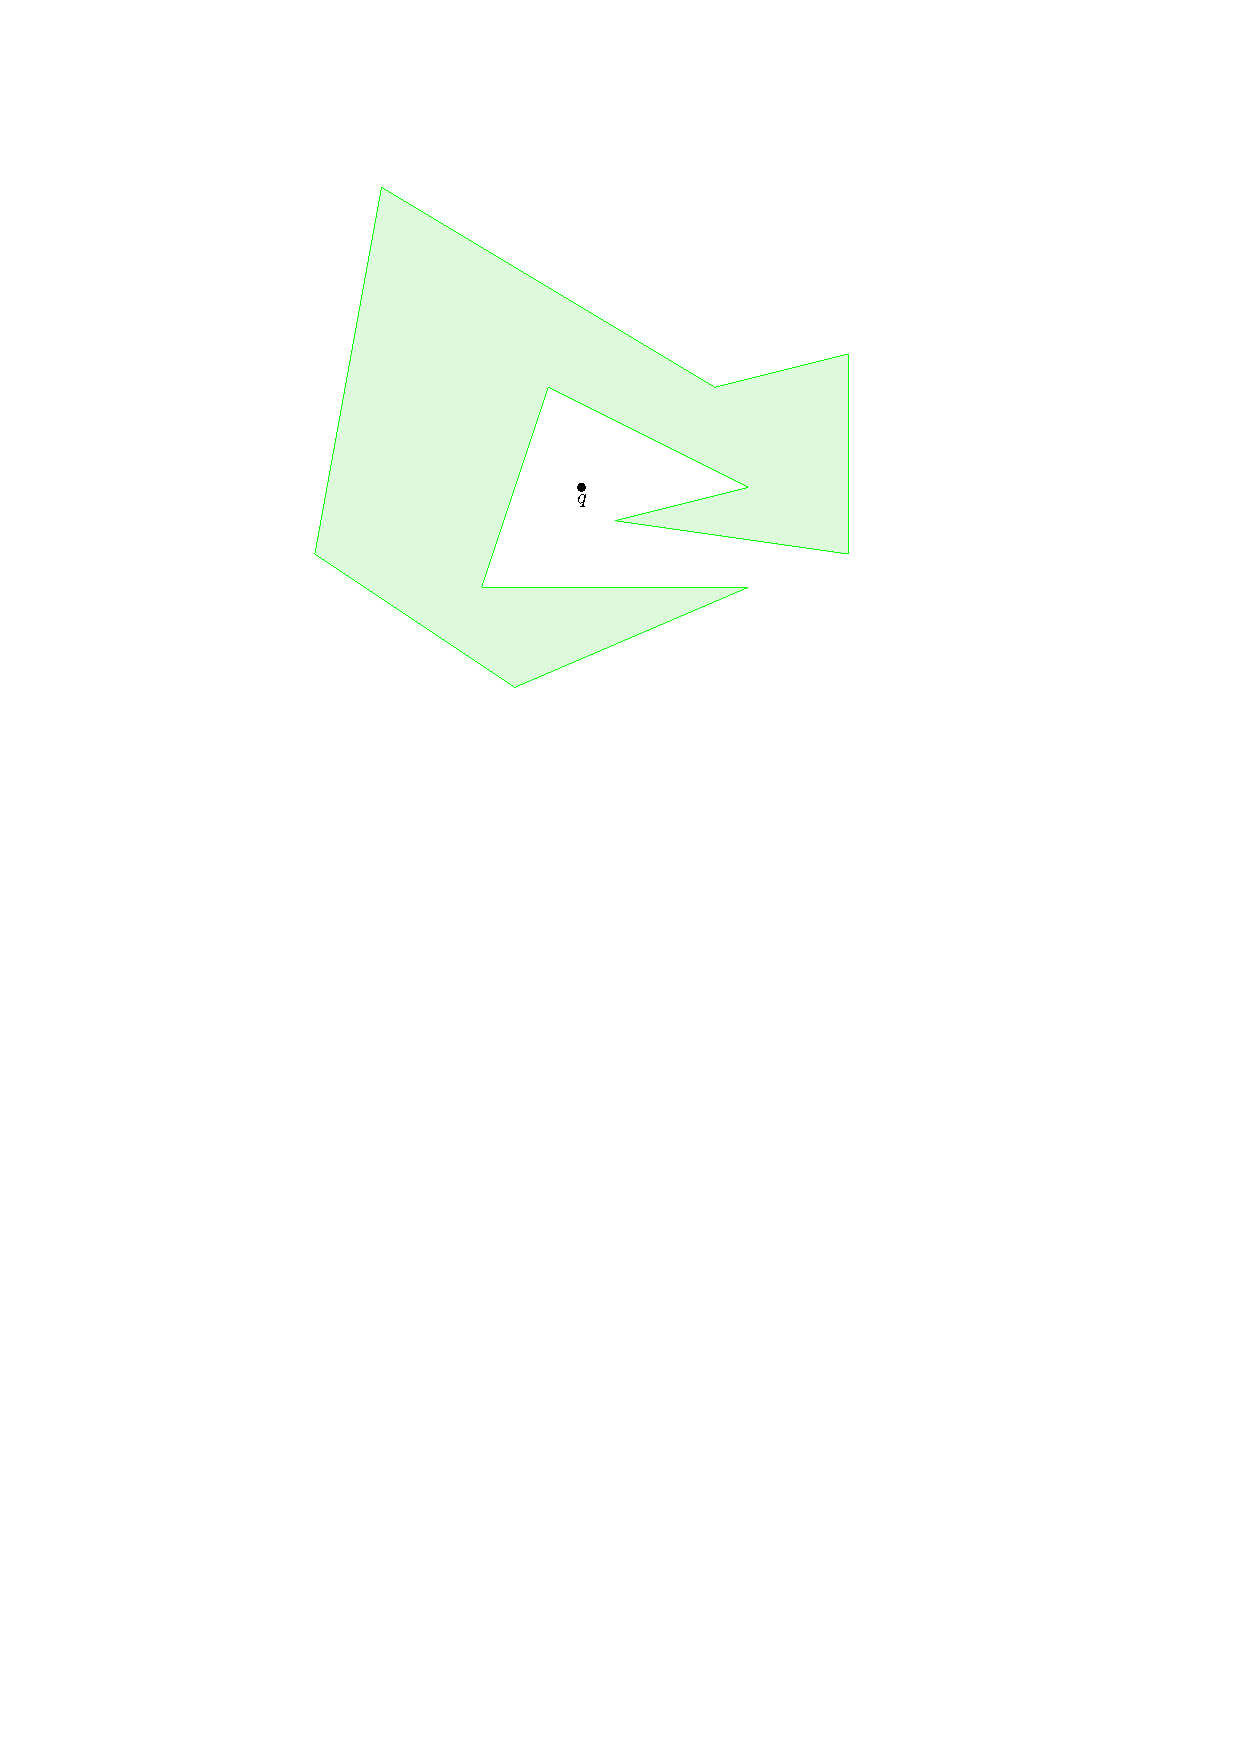
\includegraphics[width=\linewidth, height=0.5\textheight, page=1, keepaspectratio]{IPE/pip.pdf}
        \caption{Punto $q$ fuera de polígono.}
      \end{figure}
    \end{column}
    \begin{column}{0.45\textwidth}
      \begin{figure}
        \centering
        \includegraphics[width=\linewidth, height=0.5\textheight, page=2, keepaspectratio]{IPE/pip.pdf}
        \caption{Punto $q$ dentro de polígono.}
      \end{figure}
    \end{column}
  \end{columns}
\end{frame}
\begin{frame}[c]{Método del rayo}
  \begin{enumerate}
  \item Se traza una línea horizontal desde el punto hacia la derecha a lo largo del eje x.
  \end{enumerate}
  \begin{figure}
    \centering
    \includegraphics[width=\linewidth, height=0.5\textheight, page=3, keepaspectratio]{IPE/pip.pdf}
  \end{figure}
\end{frame}
\begin{frame}[c]{Método del rayo}
  \begin{enumerate}
  \item Se traza una línea horizontal desde el punto hacia la derecha a lo largo del eje x.
  \item Se cuenta el número de intersecciones con las aristas del polígono:
    \begin{enumerate}
    \item Si el número de intersecciones es par, entonces el punto está afuera del polígono.
    \item En otro caso, el punto está dentro del polígono.
    \end{enumerate}
  \end{enumerate}
  
  \begin{figure}
    \centering
    \includegraphics[width=\linewidth, height=0.5\textheight, page=4, keepaspectratio]{IPE/pip.pdf}
  \end{figure}
\end{frame}
\begin{frame}[c]{Complejidad}
  \begin{enumerate}
  \item Se traza una línea horizontal desde el punto hacia la derecha a lo largo del eje x. \textbf{O(1)}
  \item Se cuenta el número de intersecciones con las aristas del polígono:  \textbf{O(n)}
    \begin{enumerate}
    \item Si el número de intersecciones es par, entonces el punto está afuera del polígono.  \textbf{O(1)}
    \item En otro caso, el punto está dentro del polígono.  \textbf{O(1)}
    \end{enumerate}
  \end{enumerate}
  \textbf{Complejidad:} O(n)
\end{frame}
% ------------------------------------------------
% Section divider frame
\makesection{Calculando la visibilidad de un punto}

% ------------------------------------------------

\begin{frame}{El problema}
  \textbf{Non-winding polygon: O(n) algorithm}\\
  \vspace{0.5cm}
\end{frame}

% ------------------------------------------------

\begin{frame}
  % \textbf{Non-winding polygon: O(n) algorithm}\\
  \vspace{0.5cm}
  El primer paso del algoritmo es determinar si $q$ se encuentra dentro o fuera de $P$.\\
  \begin{columns}
    \begin{column}{0.45\textwidth}
      \begin{wrapfigure}{c}{0.8\textwidth}
        \centering
        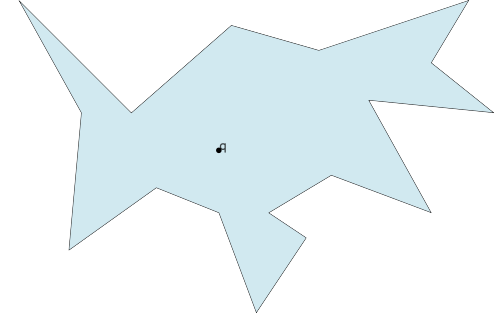
\includegraphics[width=0.8\textwidth]{imagenes/Caso1.1.png}
        \caption{q se encuentra dentro de P}
      \end{wrapfigure}
    \end{column}
    \begin{column}{0.45\textwidth}  %%<--- here
      \begin{wrapfigure}{c}{0.8\textwidth}
        \centering
        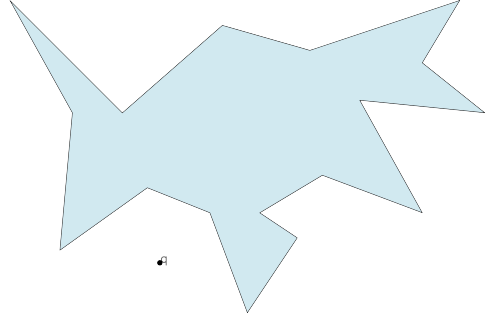
\includegraphics[width=0.8\textwidth]{imagenes/Caso1.2.png}
        \caption{q se encuentra fuera de P}
      \end{wrapfigure}
    \end{column}
  \end{columns}
  % \vspace{0.5cm}
  % Si $q$ se encuentra fuera de $P$, se construye un polígono simple $P’$ a partir de $P$ de manera que $q \in P’$ y $V(q) \subseteq P’$. Luego, el proceso para calcular el polígono de visibilidad a partir de un punto interno puede ser utilizado para calcular $V(q) \in P’$ como  $q \in P’$.\\
\end{frame}

% ------------------------------------------------

\begin{frame}[c]
  Existen dos situaciones:
  \begin{itemize}
  \item $q$ se encuentra fuera del cierre convexo de  $P$
  \item $q$ se encuentra fuera de $P$ pero dentro del cierre convexo de $P$
  \end{itemize}
\end{frame}

% ------------------------------------------------
% Double columns
\begin{frame}{}
  \begin{columns}
    \begin{column}{0.45\textwidth}
      \colheader{Si $q$ se encuentra fuera del cierre convexo de  $P$ }
      \begin{enumerate}
      \item Trazamos dos tangentes (digamos, $qv_{i}$ y $qv_{j}$) a partir de $q$ hacia el cierre convexo de $P$. 
        % \item Sea $bd(P)$ el perímetro de $P$. Notemos que todos los puntos visibles del $bd(P)$ a partir de $q$ se encuentran entre $v_{i}$ y $v_{j}$ viendo hacia q. Entonces, $bd(P’)$ consta de esta parte de $bd(P)$ entre $v_{i}$ y $v_{j}$ y dos tangentes $qv_{i}$ y $qv_{j}$.  
      \item Ahora $q$ es un punto interno de $P’$.\\
      \end{enumerate}
      \begin{block}{Observación}
        \small
        Sea $bd(P)$ el perímetro de $P$. Notemos que todos los puntos visibles del $bd(P)$ a partir de $q$ se encuentran entre $v_{i}$ y $v_{j}$ viendo hacia q.
      \end{block}
    \end{column}
    \begin{column}{0.45\textwidth}  %%<--- here
      \vspace{-1cm}
      \begin{wrapfigure}{l}{0.9\textwidth}
        \centering
        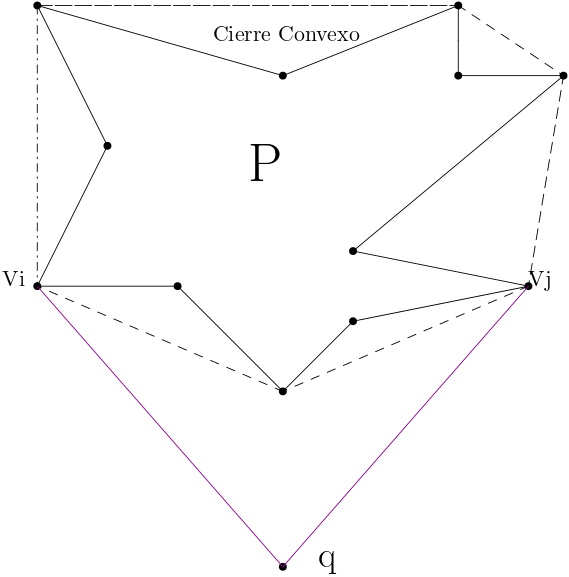
\includegraphics[width=0.9\textwidth]{imagenes/Caso01.png}
        % \caption{}
      \end{wrapfigure}
    \end{column}
  \end{columns}
\end{frame}

% Double columns
\begin{frame}{}
  \begin{columns}
    \begin{column}{0.45\textwidth}
      \begin{wrapfigure}{l}{1.1\textwidth}
        \centering
        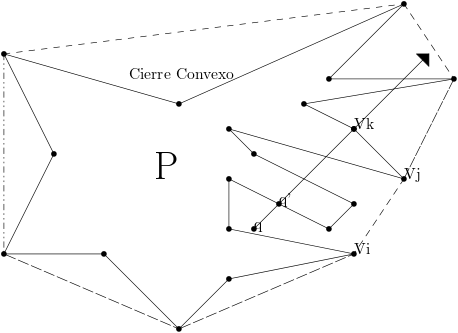
\includegraphics[width=1.1\textwidth]{imagenes/Caso02.png}
        % \caption{}
      \end{wrapfigure}
    \end{column}
    \begin{column}{0.45\textwidth}  %%<--- here
      \colheader{Si $q$ se encuentra fuera de $P$ pero dentro del cierre convexo de $P$}
      \begin{enumerate}
        % \small
        \footnotesize
      \item Trazamos una línea a partir de $q$ que pase por cualquier vértice $v_{k}$ de $P$ (denotado como $\overrightarrow{qv_{k}}$). 
      \item Sea $q’$ el punto más cercano a $q$ entre todos los puntos de las intersecciones de $\overrightarrow{qv_{k}}$ con $bd(P)$. 
      \item A partir de $q’$ recorremos $bd(P)$ en el sentido de las manecillas del reloj(y en sentido contrario) hasta que un vértice $v_{i}$ del cierre convexo (respectivamente, $v_{j}$) se alcanza.
        % Notemos que $v_{i}$ y $v_{j}$ son vértices consecutivos en el cierre convexo de $P$. Así que, $bd(P’)$ está formado por el $bd(P)$ entre $v_{i}$ y $v_{j}$ que contiene $q’$ y la arista $v_{i}v_{j}$ del cierre convexo.
      \item  Ahora, $q$ es un punto dentro de $P’$
      \end{enumerate}
    \end{column}
  \end{columns}
\end{frame}

% ------------------------------------------------

\begin{frame}[c]
  A partir de ahora, se considera que el punto $q$ es un punto interno de $P$. Por lo que, de ahora en adelante, se asume que $bd(P)$ no tiene \textit{winding} alrededor de q.
  \vspace{0.5cm}
  \begin{center}
    \textbf{El problema es calcular $V(q)$ de $P$ de $q$.}
  \end{center}
\end{frame}

% ------------------------------------------------

% \begin{frame}[c]
%   Sea $v_{0}$ el punto más cercano a $q$ entre los puntos de intersección de $bd(P)$ con la línea horizontal trazada desde $q$ a la derecha de $q$.
%   \vspace{0.5cm}
%   Asumimos que los vértices de $P$ están etiquetados de la siguiente forma: $v_{1},v_{2}, v_{3}, \dots , v_{n}$ en sentido antihorario con $v_{1}$ como el siguiente vértice en sentido antihorario después de $v_{0}$.
%   \vspace{0.5cm}
%   Asumimos que el proceso para calcular a $V(q)$ ha recorrido $bd(P)$ en el sentido contrario a las manecillas del reloj desde $v_{1}$ hasta $v_{i-1}$ y $v_{i}$ es nuestro vértice actual.
% \end{frame}

% ------------------------------------------------

\begin{frame}[c]
  \begin{block}{Observación}
    Sea $bd(v_{j}, v_{k})$ el límite en sentido antihorario de $P$ desde $v_{j}$ hasta $v_{k}$.    
  \end{block}
  \vspace{0.5cm}
  También asumimos que los vértices (y los puntos finales de las \textit{aristas construidas}) en $bd(v_{0} v_{i-1})$, las cuales se encuentran para ser visibles desde $q$ por el procedimiento, son colocadas en un stack en el orden en que son encontradas, donde $v_{0}$ y $v_{i-1}$ están en la parte inferior y superior del stack, respectivamente.\\  
\end{frame}

% ------------------------------------------------

\begin{frame}[c]
  Contamos con los siguientes casos
  \begin{center}
    \begin{enumerate}
    \item El vértice $v_{i}$ se encuentra a la izquierda de $\overrightarrow{qv_{i-1}}$
    \item El vértice $v_{i}$ se encuentra a la derecha de $\overrightarrow{qv_{i-1}}$
      \begin{enumerate}
      \item El vértice $v_{i}$ se encuentra a la derecha de $\overrightarrow{v_{i-2}v_{i-1}}$
      \item El vértice $v_{i}$ se encuentra a la izquierda de $\overrightarrow{v_{i-2}v_{i-1}}$
      \end{enumerate}
    \end{enumerate}
  \end{center}
\end{frame}

% ------------------------------------------------

\begin{frame}{Caso 1}
  \textbf{El vértice $v_{i}$ se encuentra a la izquierda de $\overrightarrow{qv_{i-1}}$}\\
  \vspace{0.5cm}
  \begin{columns}
    \begin{column}{0.45\textwidth}
      Como $v_{i}$ y los vértices y puntos en el stack se encuentran ordenados por el ordenamiento  angular respecto a $q$, $v_{i}$ es ingresado al stack.
    \end{column}
    \begin{column}{0.45\textwidth}  %%<--- here
      \vspace{-1.5cm} % Ajuste vertical aquí
      \begin{wrapfigure}{l}{0.9\textwidth}
        \centering
        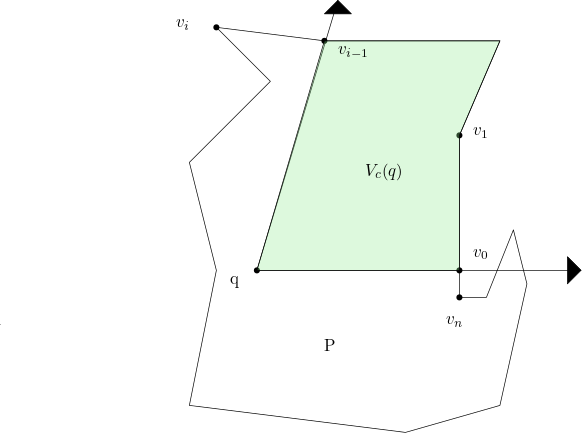
\includegraphics[width=0.9\textwidth]{imagenes/Caso2.4a.png}
        % \caption{}
      \end{wrapfigure}
    \end{column}
  \end{columns}
\end{frame}

% ------------------------------------------------

\begin{frame}{Caso 2}
  \textbf{El vértice $v_{i}$ se encuentra a la derecha de $\overrightarrow{qv_{i-1}}$}\\
  \vspace{0.5cm}
  \begin{columns}
    \begin{column}{0.45\textwidth}
      Puede observarse que $v_{i-1}$ y $v_{i}$ no pueden ser visibles por $q$ ya que $qv_{i}$ es intersectado por $bd(v_{0}, v_{i-1})$ o $qv_{i-1}$ es intersectado por $bd(v_{i+1}, v_{n})$ 
    \end{column}
    \begin{column}{0.45\textwidth}  %%<--- here
      \vspace{-1.5cm} % Ajuste vertical aquí
      \begin{wrapfigure}{l}{0.95\textwidth}
        \centering
        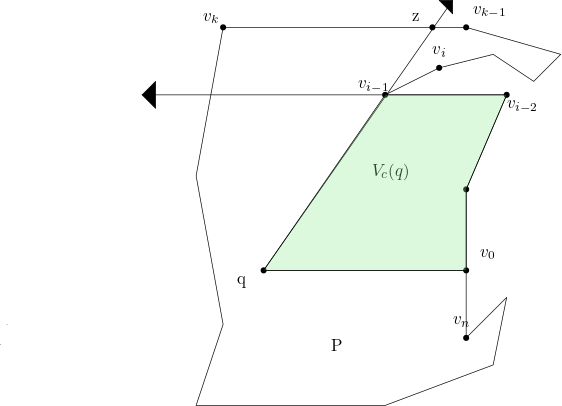
\includegraphics[width=0.95\textwidth]{imagenes/Caso2.4b.png}
        % \caption{}
      \end{wrapfigure}
    \end{column}
  \end{columns}
\end{frame}

% ------------------------------------------------

\begin{frame}{Caso 2a}
  \textbf{El vértice $v_{i}$ se encuentra a la derecha de $\overrightarrow{v_{i-2}v_{i-1}}$}\\
  \vspace{0.5cm}
  \begin{columns}
    \begin{column}{0.45\textwidth}
      El vértice $v_{i}$ y algunos de los vértices subsecuentes de $v_{i}$ (que serán revisados) no son visibles desde $q$.\\
      \vspace{0.5cm}
      Sea $v_{k-1}v_{k}$ la primer arista desde $v_{i+1}$ en $bd(v_{i+1},v_{n})$, en sentido antihorario de manera que $v_{k+1}v_{k}$ intersecta $\overrightarrow{qv_{i-1}}$.\\
      \vspace{0.5cm}
      Sea $z$ el punto de intersección.
    \end{column}
    \begin{column}{0.45\textwidth}  %%<--- here
      \vspace{-1.5cm} % Ajuste vertical aquí
      \begin{wrapfigure}{l}{0.95\textwidth}
        \centering
        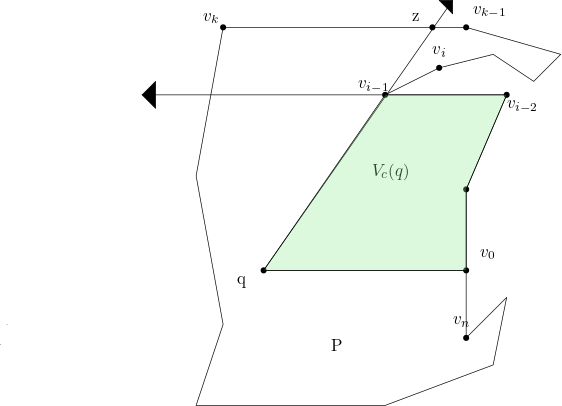
\includegraphics[width=0.95\textwidth]{imagenes/Caso2.4b.png}
        % \caption{}
      \end{wrapfigure}
    \end{column}
  \end{columns}
\end{frame}

% ------------------------------------------------

\begin{frame}{Caso 2a}
  \textbf{El vértice $v_{i}$ se encuentra a la derecha de $\overrightarrow{v_{i-2}v_{i-1}}$}\\
  \vspace{0.5cm}
  \begin{columns}
    \begin{column}{0.45\textwidth}
      Veamos que $v_{k}$ se encuentra a la izquierda de $\overrightarrow{qv_{v_{i-1}}}$ ya que $bd(P)$ does not wind around $q$. Entonces, ningún vértice de $bd(v_{i}, v_{v_{k-1}})$ es visible desde $q$ y por consiguiente, $z$ es el siguiente punto de $v_{i-1}$ en $bd(v_{i-1}, v_{n})$ visible desde $q$. Así que, $v_{i}z$ es una \textit{arista construida} de $V(q)$, donde $q$, $v_{i-1}$ y $z$ son puntos colineales.
    \end{column}
    \begin{column}{0.45\textwidth}  %%<--- here
      \vspace{-1.5cm} % Ajuste vertical aquí
      \begin{wrapfigure}{l}{0.95\textwidth}
        \centering
        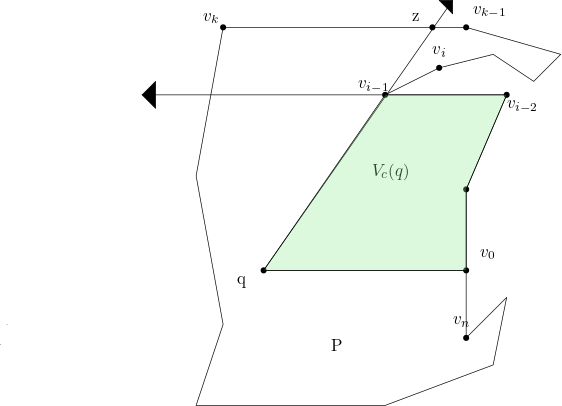
\includegraphics[width=0.95\textwidth]{imagenes/Caso2.4b.png}
        % \caption{}
      \end{wrapfigure}
    \end{column}
  \end{columns}
\end{frame}

% ------------------------------------------------

\begin{frame}{Caso 2b}
  \textbf{El vértice $v_{i}$ se encuentra a la izquierda de $\overrightarrow{v_{i-2}v_{i-1}}$}\\
  \vspace{0.5cm}
  \begin{columns}
    \begin{column}{0.45\textwidth}
      \small
      El vértice $v_{i-1}$ y algunos de los vértices anteriores de $v_{i}$ (quien está actualmente en el stack) no son visibles desde $q$. Sacamos a $v_{i}$ del stack. \\
      \vspace{0.5cm}
      Sea $u$ vértice que se encuentra en la parte superior del stack. La arista $v_{i-1}v_{i}$ es conocida como \textit{arista frontal}. Mientras $v_{i-1}v_{i}$ intersecta $uq$ y $u$ es un vértice de $P$, realizamos pop al stack.\\
    \end{column}
    \begin{column}{0.45\textwidth}  %%<--- here
      \vspace{-1.5cm}
      \begin{wrapfigure}{l}{0.95\textwidth}
        \centering
        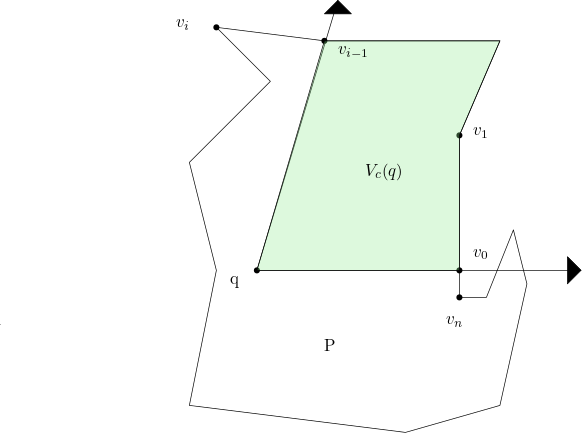
\includegraphics[width=0.95\textwidth]{imagenes/Caso2.4a.png}
        % \caption{}
      \end{wrapfigure}
    \end{column}
  \end{columns}
\end{frame}

% ------------------------------------------------

\begin{frame}[c]
  Después de ejecutar el backtracking, pueden suceder dos situaciones
  \begin{center}
    \begin{enumerate}
    \item [i.] $v_{i-1}v_{i}$ no intersecta $uq$
    \item [ii.] $v_{i-1}v_{i}$ intersecta $uq$
    \end{enumerate}
  \end{center}
\end{frame}

% ------------------------------------------------
% Double columns
\begin{frame}{Caso 2b.i}
  \textbf{$v_{i-1}v_{i}$ no intersecta $uq$}\\ 
  \begin{columns}
    \begin{column}{0.45\textwidth}
      Si $v_{i+1}$ se encuentra a la derecha de $\overrightarrow{qv_{i}}$, el backtracking continua con $v_{i}v_{i+1}$ como la \textit{arista frontal} actual.
      \begin{wrapfigure}{c}{0.6\textwidth}
        \centering
        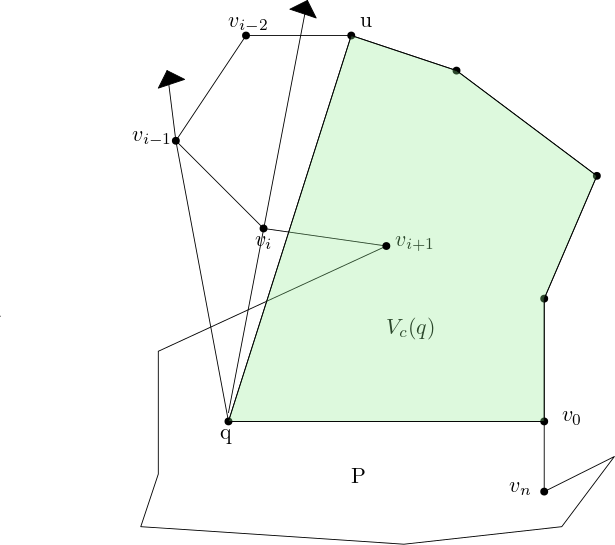
\includegraphics[width=0.6\textwidth]{imagenes/Caso2.5b.png}
        % \caption{}
      \end{wrapfigure}
    \end{column}
    \begin{column}{0.45\textwidth}  %%<--- here
      De otra forma, $v_{i+1}$ se encuentra a la izquierda de $\overrightarrow{qv_{i}}.$
      \begin{wrapfigure}{c}{0.5\textwidth}
        \centering
        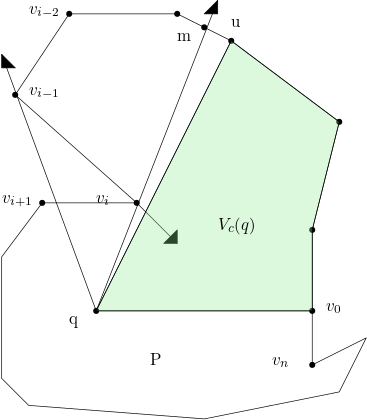
\includegraphics[width=0.5\textwidth]{imagenes/Caso2.6a.png}
        % \caption{}
      \end{wrapfigure}
    \end{column}
  \end{columns}
\end{frame}

% % ------------------------------------------------

\begin{frame}{Caso 2b.i}
  \textbf{$v_{i-1}v_{i}$ no intersecta $uq$}\\
  \vspace{0.5cm}
  \begin{columns}
    \begin{column}{0.45\textwidth}
      Sea $m$ el punto de intersección de $\overrightarrow{qv_{i}}$ con la arista del polígono que contiene $u$.\\
      \vspace{0.5cm}
      Si $v_{i+1}$ se encuentra a la derecha de $\overrightarrow{v_{i-1}v_{i}}$, entonces termina el backtracking.
    \end{column}
    \begin{column}{0.45\textwidth}  %%<--- here
      \vspace{-2.5cm}
      \begin{wrapfigure}{l}{0.75\textwidth}
        \centering
        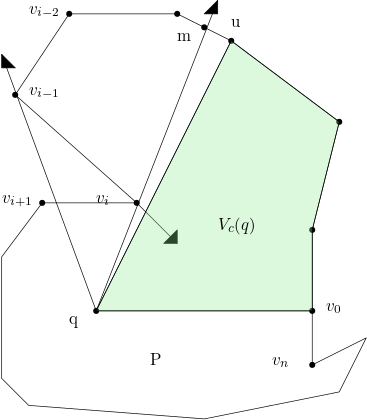
\includegraphics[width=0.75\textwidth]{imagenes/Caso2.6a.png}
        % \caption{}
      \end{wrapfigure}
    \end{column}
  \end{columns}
\end{frame}

% ------------------------------------------------

\begin{frame}{Caso 2b.i}
  \textbf{$v_{i-1}v_{i}$ no intersecta $uq$}\\
  \vspace{0.5cm}
  \begin{columns}
    \begin{column}{0.45\textwidth}
      Ingresamos $m$ y $v_{i+1}$ al stack y $v_{i+1}$ se convierte en el nuevo $v_{i}$.\\
      \vspace{0.5cm}
      Si $v_{i+1}$ se encuentra a la izquierda de $\overrightarrow{v_{i-1}v_{i}}$, revisamos $bd(v_{i+1}, v_{n})$ desde $v_{i+1}$ hasta que un vértice $v_{k}$ es encontrado de manera que la arista $v_{k-1}v_{k}$ intersecta $mv_{i}$. El backtracking continua con $v_{k-1}v_{k}$ como la \textit{arista frontal} actual.    
    \end{column}
    \begin{column}{0.45\textwidth}  %%<--- here
      \vspace{-1.5cm}
      \begin{wrapfigure}{c}{1.1\textwidth}
        \centering
        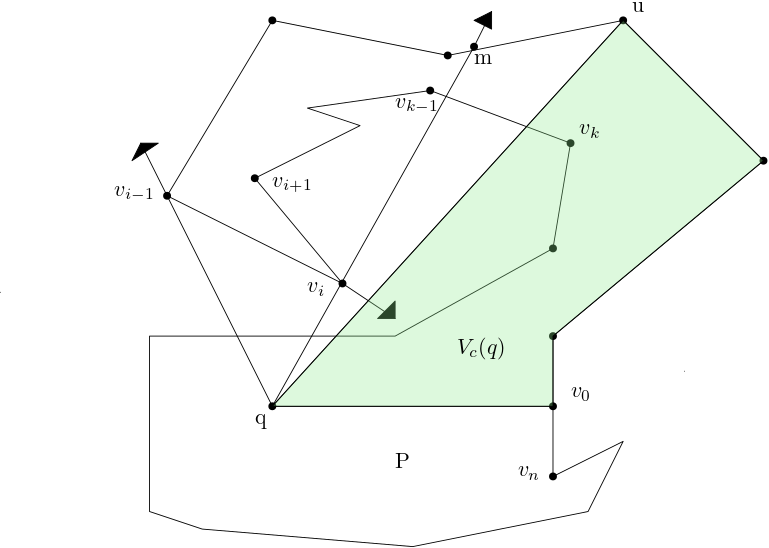
\includegraphics[width=1.1\textwidth]{imagenes/Caso2.6b.png}
        % \caption{}
      \end{wrapfigure}
    \end{column}
  \end{columns}
\end{frame}

%%%%%%%%%%%%%%%%%%%% Caso 2b.ii %%%%%%%%%%%%%%%%%%%%
% ------------------------------------------------

\begin{frame}{Caso 2b.ii}
  \textbf{$v_{i-1}v_{i}$ intersecta $uq$}\\
  \vspace{0.5cm}
  \begin{columns}
    \begin{column}{0.45\textwidth}
      $u$ no es un vértice de $P$. Sea $w$ el vértice que se encuentra justo debajo de $u$ en el stack. Por lo que, $uw$ es una \textit{arista construida}\\
      \vspace{0.5cm}
    \end{column}
    \begin{column}{0.45\textwidth}  %%<--- here
      \vspace{-3cm}
      \begin{wrapfigure}{l}{0.85\textwidth}
        \centering
        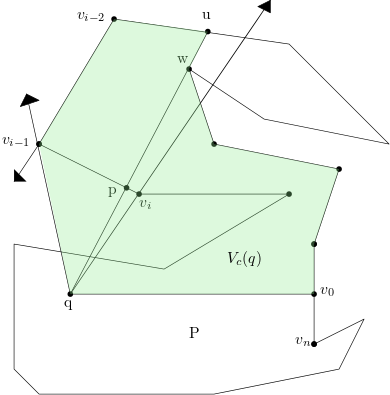
\includegraphics[width=0.85\textwidth]{imagenes/Caso2.7a.png}
        % \caption{}
      \end{wrapfigure}
    \end{column}
  \end{columns}
\end{frame}

% ------------------------------------------------

\begin{frame}{Caso 2b.ii}
  \textbf{$v_{i-1}v_{i}$ intersecta $uq$}\\
  \vspace{0.5cm}
  \begin{columns}
    \begin{column}{0.45\textwidth}
      Sea $p$ el punto de intersección de $uq$ y $v_{i-1}v_{i}$. Si $p \in qw$, la visibilidad de ambos, $u$ y $w$ desde $q$ esta bloqueada por $v_{i-1}v_{i}$. Vaciamos el stack.\\
      \vspace{0.5cm}
      El backtracking continua y $v_{i-1}v_{i}$ permanece como la \textit{arista frontal}.\\
      \vspace{0.5cm}
    \end{column}
    \begin{column}{0.45\textwidth}  %%<--- here
      \vspace{-3cm}
      \begin{wrapfigure}{l}{0.85\textwidth}
        \centering
        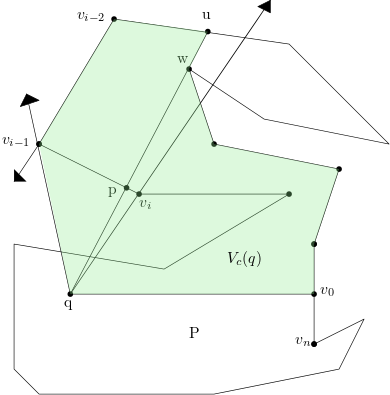
\includegraphics[width=0.85\textwidth]{imagenes/Caso2.7a.png}
        % \caption{}
      \end{wrapfigure}
    \end{column}
  \end{columns}
\end{frame}

% ------------------------------------------------

\begin{frame}{Caso 2b.ii}
  \textbf{$v_{i-1}v_{i}$ intersecta $uq$}\\
  \vspace{0.5cm}
  \begin{columns}
    \begin{column}{0.45\textwidth}
      De otra forma, $v_{i-1}v_{i}$ ha intersectado $uw$ como $p$ pertenece a $uw$.\\
      \vspace{0.5cm}
      Checamos $bd(v_{i+1, v_{n}})$ desde $v_{i+1}$ hasta encontrar un vértice $v_{k}$ tal que la arista $v_{k-1}v_{k}$ ha sido intersectada por $wp$ en algún punto (digamos, $z$). Así que, todo $bd(w,z)$(a excepción de $w$ y $z$) no es visible por $q$. Vaciamos el stack.\\
      \vspace{0.5cm}
    \end{column}
    \begin{column}{0.45\textwidth}  %%<--- here
      \vspace{-2.5cm}
      \begin{wrapfigure}{l}{1\textwidth}
        \centering
        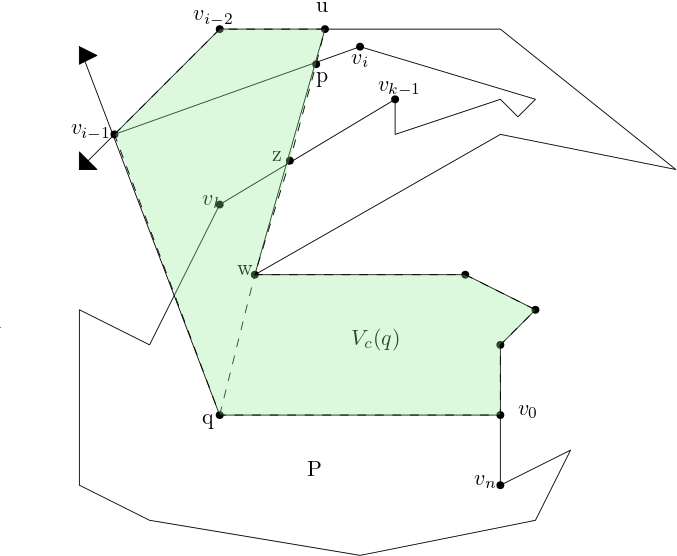
\includegraphics[width=1\textwidth]{imagenes/Caso2.7b.png}
        % \caption{}
      \end{wrapfigure}
    \end{column}
  \end{columns}
\end{frame}

% ------------------------------------------------

\begin{frame}{Caso 2b.ii}
  \textbf{$v_{i-1}v_{i}$ intersecta $uq$}\\
  \vspace{0.2cm}
  \begin{columns}
    \begin{column}{0.45\textwidth}
      \footnotesize
      Ingresamos a $z$ y a $v_{k}$ al stack. Por lo que, $v_{k+1}$ se convierten en el nuevo $v_{i}$. Puede suceder que la \textit{arista construida} que termina en $u$ (digamos, uu’) haya sido calculada por el Caso 2b al final de la fase de backtracking. Esto significa que el vértice u’ es el último vértice en el stack que va a ser sacado en la fase de backtracking actual. Por lo tanto, $q$, $w$ y $z$ no son colineales. Los sacamos del stack y notemos que nos encontramos la primera situación del backtracking actual.\\
      \vspace{0.5cm}
    \end{column}
    \begin{column}{0.45\textwidth}  %%<--- here
      \vspace{-2cm}
      \begin{wrapfigure}{l}{1\textwidth}
        \centering
        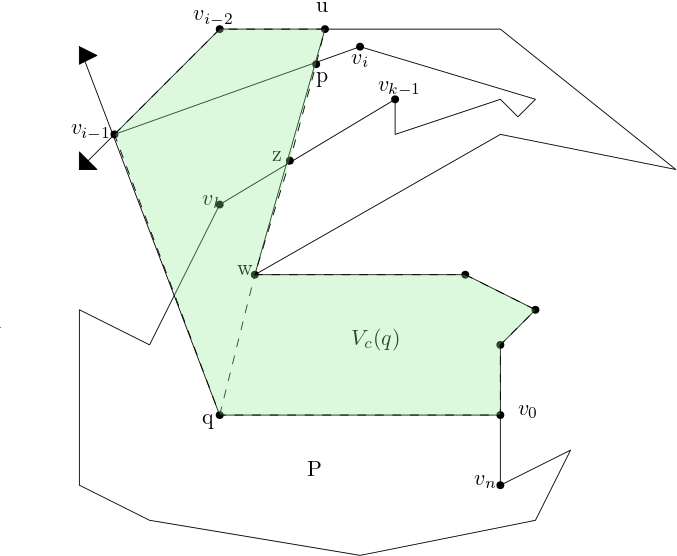
\includegraphics[width=1\textwidth]{imagenes/Caso2.7b.png}
        % \caption{}
      \end{wrapfigure}
    \end{column}
  \end{columns}
\end{frame}

% ------------------------------------------------

\makesection{Algoritmo para calcular $V(q)$}
\subsection{Algoritmo}
\subsection{Complejidad}

% ------------------------------------------------
% Algoritmo presentado formalmente
\begin{frame}{Algoritmo para calcular $V(q)$}
  \begin{enumerate}
  \item Ingresamos a $v_{1}$ al stack y $i := i + 1$. Si $i = n + 1$ \textit{Ir al Paso 8.}
  \item Si $v_{i}$ se encuentra a la izquierda de $\overrightarrow{qv_{i-1}}$ entonces \textit{Ir al Paso 1}
  \item Si $v_{i}$ se encuentra a la derecha de $\overrightarrow{qv_{i-1}}$ y $\overrightarrow{v_{i-2}v_{i-1}}$ entonces
    \begin{enumerate}
    \item Checar desde $v_{i+1}$ en sentido antihorario hasta encontrar un vértice $v_{k}$ tal que $v_{k-1}v_{k}$ intersecta $\overrightarrow{qv_{i-1}}$. Sea $z$ el punto de intersección.
    \item Ingresamos $z$ al stack. $i := k$ e \textit{Ir al Paso 1.}
    \end{enumerate}
  \item Si $v_{i}$ se encuentra a la derecha de $\overrightarrow{qv_{i-1}}$ y a la izquierda de $\overrightarrow{v_{i-2}v_{i-1}}$ entonces
    \begin{enumerate}
    \item Sea $u$ el elemento que se encuentra en la parte superior del stack. Realizamos \textit{pop} al stack.
    \item Mientras $u$ sea un vértice y $v_{i-1}v_{i}$ intersecte $uq$, realizamos \textit{pop} al stack. 
    \end{enumerate}
  \end{enumerate}
\end{frame}
\begin{frame}{}
  \begin{enumerate}
    \setcounter{enumi}{4} 
  \item Si $v_{i-1}v_{i}$ no intersecta $uq$ entonces
    \begin{enumerate}
    \item Si $v_{i+1}$ se encuentra a la derecha de $\overrightarrow{qv_{i}}$ entonces $i := i + 1$ e \textit{Ir al Paso 4b.}
    \item Sea $m$ el punto de intersección de $\overrightarrow{qv_{i}}$ y la arista que contiene a $u$. Si $v_{i+1}$ se encuentra a la derecha de $\overrightarrow{v_{i-1}v_{i}}$ entonces ingresamos $m$ al stack y \textit{vamos al Paso 1.}
    \item Checamos desde $v_{i+1}$ en orden antihorario hasta encontrar un vértice $v_{k}$ tal que $v_{k-1}v_{k}$ intersecte $mv_{i}$. Asignamos $k$ a $i$ y \textit{vamos al Paso 4b.}
    \end{enumerate}
  \item Sea $w$ el vértice que se encuentra justo debajo de $u$ en el stack. Sea $p$ el punto de intersección entre $v_{i-1}v_{i}$ y $uq$. Si $p \in qw$ o $q$, $w$ y $u$ no son colineales entonces realizamos \textit{pop} al stack y \textit{vamos al paso 4b}.
  \item Checamos desde $v_{i+1}$ en sentido antihorario hasta encontrar un vértice $v_{k}$ tal que $v_{k-1}v_{k}$ intersecte $wp$. Insertamos el punto de intersección al stack, asignamos $k$ a $i$ y \textit{vamos al Paso 1.}
  \item Generamos $V(q)$ sacando todos los vértices y puntos del stack y nos detenemos.
  \end{enumerate}
\end{frame}



% ------------------------------------------------

\begin{frame}{Complejidad del algoritmo}
  \begin{block}{Invariante}
    El algoritmo mantiene una invariante de que los vértices y puntos en la pila en cualquier etapa están ordenados angularmente con respecto a q.
  \end{block}    
  \vspace{0.5cm}
  Revisemos paso a paso la complejidad del algoritmo
  \begin{enumerate}
  \item Inicialización: $O(1)$
  \item La ejecución recorre los n vértices una vez y para cada vértice se realizan operaciones en el stack: $O(n)$
  \end{enumerate}
  \begin{center}
    \textbf{Complejidad Total: $O(n)$}
  \end{center}
\end{frame}

% ------------------------------------------------

% \begin{frame}{Teorema}
%   \begin{block}{Teorema}
%     El polígono de visibilidad $V(q)$ de un punto dado $q$ dentro de un polígono simple de $n$ lados $P$ de puede ser calculado en tiempo $O(n)$.
%   \end{block}
% \end{frame}

% % ----------------------------------------------------------------------------------------
% Final PAGE
% Set the text that is showed on the final slide
\finalpagetext{Gracias por su atención}
% ----------------------------------------------------------------------------------------
\makefinalpage
% ----------------------------------------------------------------------------------------
\end{document}
